\chapter{Designing the Data Capture System}
To obtain data for the Extended Kalman Filter, a data-capture system needed to be designed. Since the data sources have been identified as multiple video sources and a 9-DOF IMUthe equipment has been selected as follows. 

\section{GoPro Hero Session Camera}
Due to the availability of GoPro Hero Session cameras the wearable motion capture system was designed with these in mind. These cameras only take up a volume of $250cm^3$ and has a square housing measuring $6.3cm$ on all sides. The following figure presents a visual of the camera.

\begin{figure}[!ht] 
\captionsetup{width=\linewidth, font=small}  
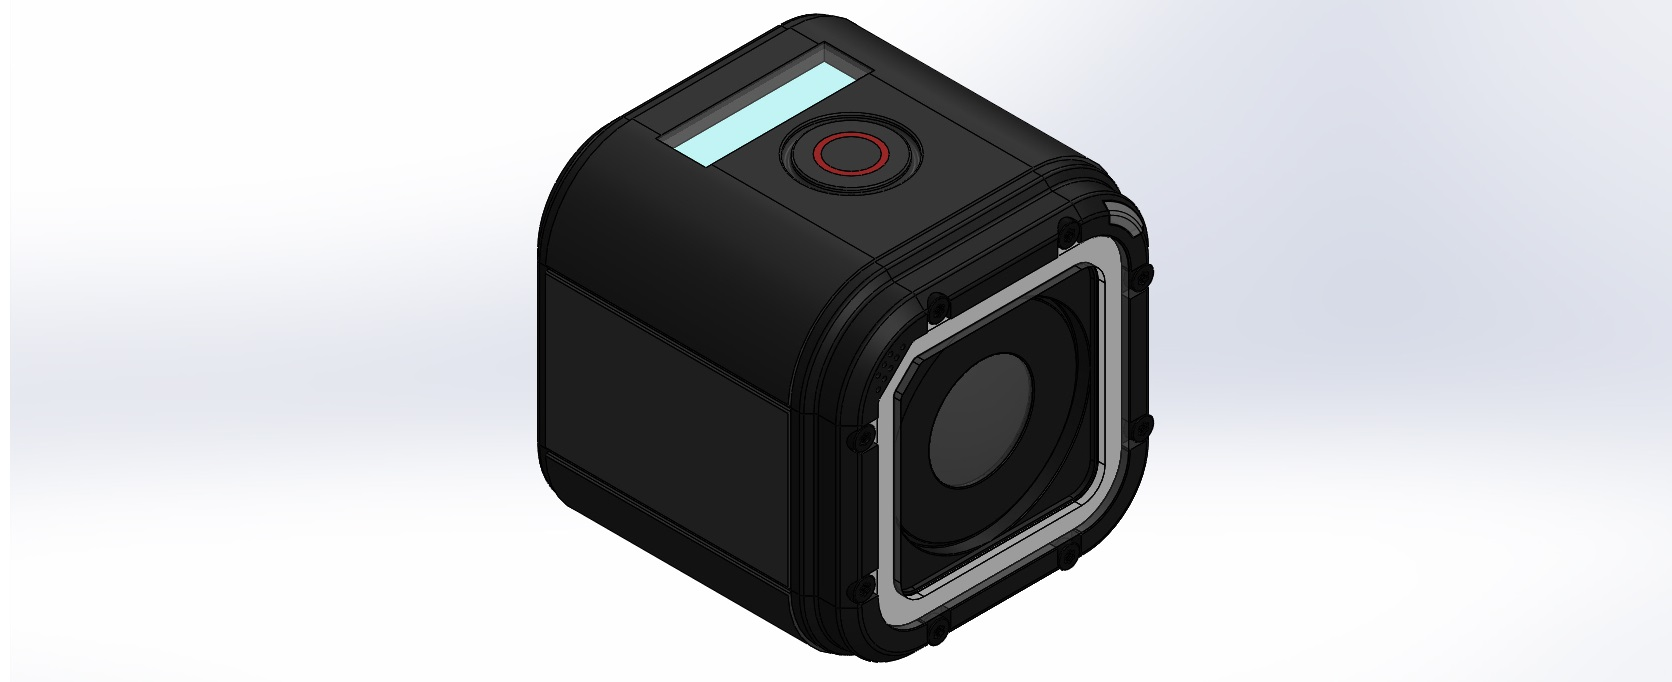
\includegraphics[width=\linewidth]{figures/GoProHero4Session.JPG}
\caption{3D CAD rendering of the GoPro Hero Session action camera}
\label{fig:GoProHero4Session}
\end{figure}

The camera can capture videos at a variety of frame rates and a variety of resolutions. These settings are limited as the software that controls the camera is proprietary.

These set frame rates and resolutions are presented in the table below.
\begin{table}[!ht]
\centering
\caption{Possible frame rate and resolution combinations on the GPHS camera}
\label{framesres}
\begin{tabular}{ll}
Resolution  & Frame Rates                             \\
1920 x 1440 & 30 fps, 25 fps                          \\
1920 x 1080 & 60 fps, 50 fps, 48 fps, 30 fps, 25 fps  \\
1280 x 960  & 60 fps, 50 fps, 30 fps, 25 fps          \\
1280 x 720  & 100 fps, 60 fps, 50 fps, 30 fps, 25 fps \\
848 x 480   & 120 fps, 100 fps                       
\end{tabular}
\end{table}

The relative motion of the lower limbs appeared to move rapidly and therefore the highest possible framerate with the best resolution was chosen. The camera was therefore configured to record at 100Hz and a resolution of 1280 x 720 pixels. This was chosen as the quality of the 848 x 480 video was simply to low to analyse using computer algorithms.

The camera also has the ability to record using a normal lens or a wide angle lens. The field of view of the camera greatly increases with the wide angle lens but its focal length decreases proportionally. The wide lens also produces more distortion when compared to the normal lens. Due to the relatively narrow area of capture needed the camera was configured to use the normal lens as it would decrease distortion without compromising the area of interest.
   

\section{Camera Mount Design}

Some initial work on modelling a housing for the camera was completed by the Mechatronics Lab. This was a 2 part 3D printable enclosure with no mounting points. The enclosure is pictured below.

\begin{figure}[!ht] 
\captionsetup{width=0.6\linewidth, font=small}  
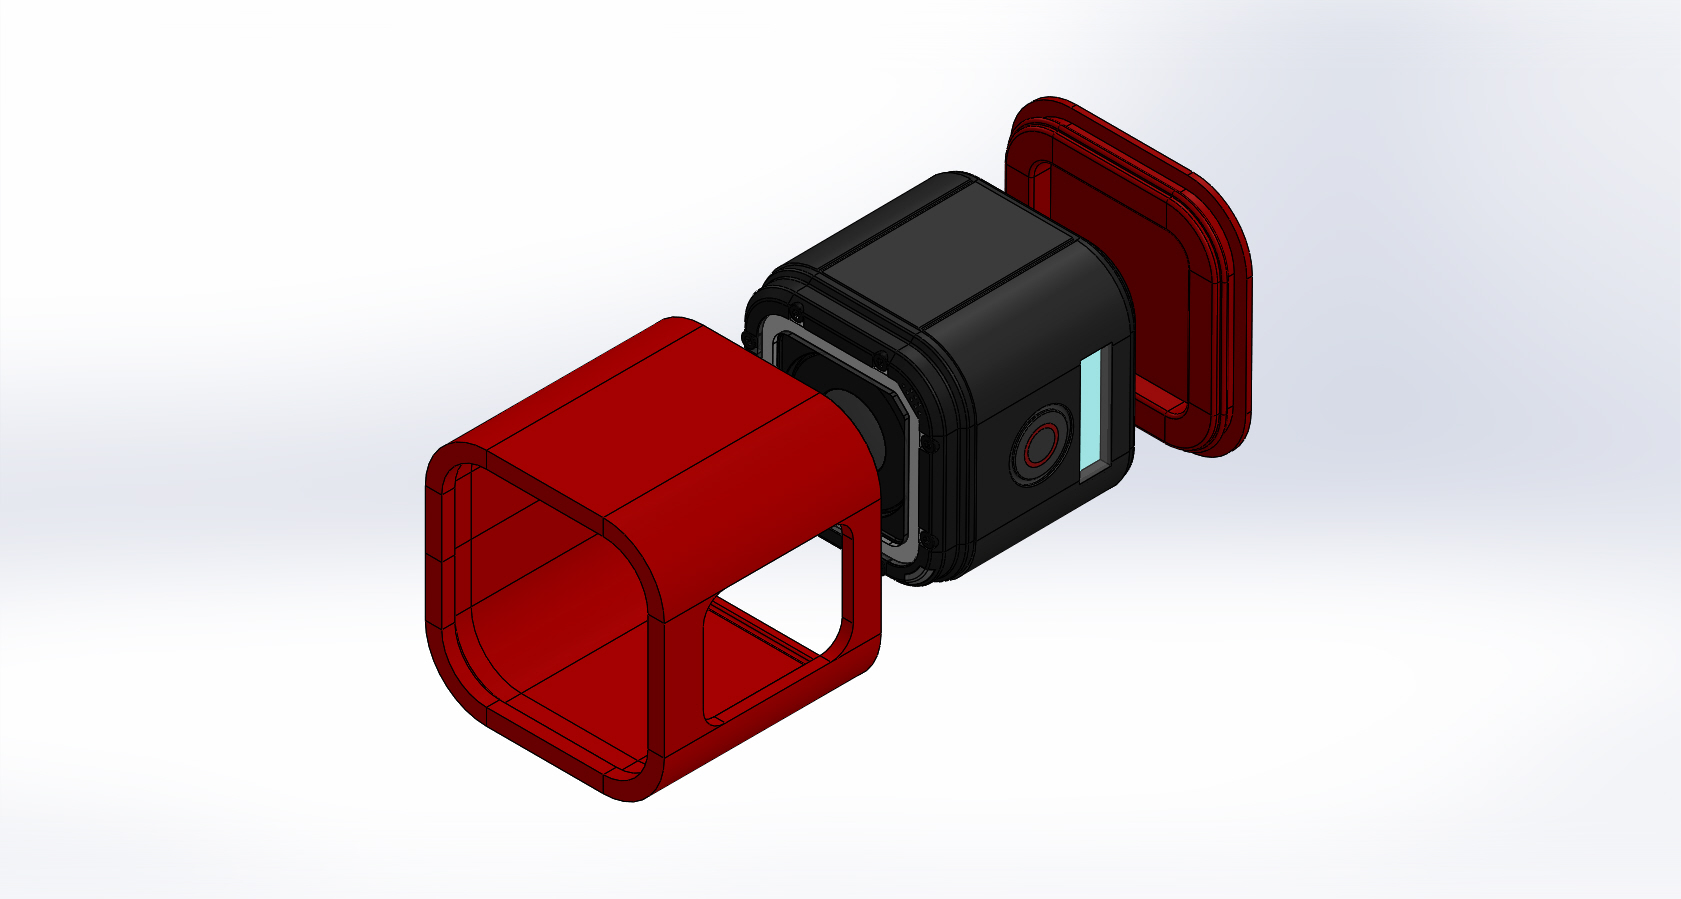
\includegraphics[width=0.6\linewidth]{figures/sylvanexploded.JPG}
\caption{Initial camera enclosure designed by the mechatronics lab}
\label{fig:sylvanexploded}
\end{figure}

This model was heavily modified using Dassault Systems SOLIDWORKS software to enclose 2 cameras mounted side by side. The bracket also needed a mounting point to join to the chest mount. Finally the bracket needed to be lightweight, provide access to the camera controls and not obscure the built in status screen of the cameras. The following figure shows the final dual camera bracket that was 3D printed.

\begin{figure}[!ht] 
\captionsetup{width=\linewidth, font=small}  
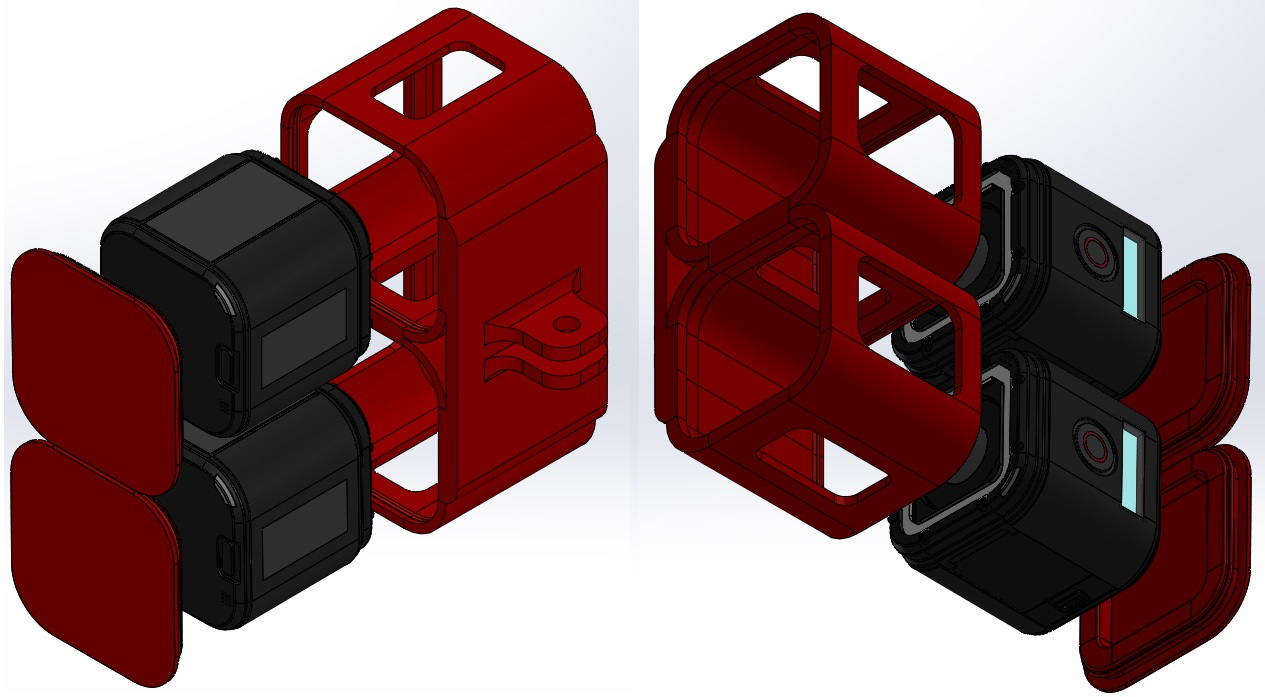
\includegraphics[width=\linewidth]{figures/stereoholder.JPG}
\caption{Final dual camera enclosure designed by the author}
\label{fig:stereoholder}
\end{figure}



\section{Vision Calibration}
In order to obtain accurate positional information from the video cameras calibration was performed. MATLAB has a built in stereo camera calibration application that can calibrate a set of cameras and create an object containing all the essential parameters, including the individual camera intrinsics.

To calibrate the cameras pictures of a white and black chequerboard is fed in to the calibration application that then mathematically determines the camera parameters. In order to make this process more efficient a video of the the moving chequerboard was taken and various frames of importance extracted using a simple MATLAB script. 



